\apendice{Documentación de usuario}
\section{Introducción}
Este manual explica los requisitos necesarios para utilizar correctamente los dispositivos y el programa, así como las instrucciones de instalación y uso.
\section{Requisitos de usuarios}
A continuación se muestra una tabla con los requisitos mínimos necesarios para ejecutar la aplicación a través de \textit{Meta Quest Link}.
\begin{table}[H]
\centering
\scalebox{0.85}{
\begin{tabular}{@{}p{9em} p{12em} p{12em}@{}}
\toprule
\textbf{Componente} & \textbf{Requisitos mínimos} & \textbf{Comentarios} \\
\midrule
CPU & Intel i5‑4590 o AMD Ryzen 5 1500X o superior &\\
\hline
RAM & 8GB o superior & Memoria RAM recomendada para ejecutar entornos en VR. \\
\hline
GPU & Tarjeta gráfica con soporte para codificación H.264/H.265 & Recomendado: NVIDIA GTX 970, AMD RX 570 o superior. \\
\hline
Sistema operativo & Windows 10 o Windows 11 (64 bits) & Compatible con la aplicación de escritorio de Meta Quest Link. \\
\hline
USB & Puerto USB‑C o USB3.0 & . \\
\hline
Almacenamiento & 5GB de espacio libre & Necesario para instalar el software de Meta Quest Link y la aplicación VRRecoveryGym\\
\bottomrule
\end{tabular}
}
\caption[Requisitos mínimos PC para Meta Quest Link]{Requisitos mínimos del sistema para ejecutar el proyecto mediante \textit{Meta Quest Link}.\cite{metaRequisitos}}
\label{tab:req-meta-quest-link}
\end{table}

\subsection{Instalación de \textit{Meta Quest Link}}

Para poder ejecutar el sistema de rehabilitación en unas gafas \textit{Meta Quest 2} conectadas al ordenador, es necesario utilizar la herramienta \textit{Meta Quest Link}, que permite el uso del visor como pantalla de realidad virtual para aplicaciones instaladas en el PC.

A continuación, se indican los pasos que debe seguir el usuario para instalar y conectar correctamente el dispositivo:

\begin{enumerate}
    \item \textbf{Descargar el software oficial}: Acceder a la página \href{https://www.meta.com/quest/setup/}{oficial} y descargar la aplicación \textit{Meta Quest Link} para Windows.

    \item \textbf{Instalar la aplicación}: Ejecutar el instalador descargado y seguir las instrucciones en pantalla para completar la instalación.

    \item \textbf{Conectar las gafas al ordenador}:
    \begin{itemize}
        \item \textbf{Opción por cable}: Conectar las gafas al PC mediante un cable USB-C.
        \item \textbf{Opción inalámbrica}: Conectarse por Wi-Fi mediante la función \textit{Air Link}. Para ello, tanto el visor como el ordenador deben estar en la misma red local y con una buena conexión (preferiblemente a través de router 5 GHz).
    \end{itemize}

    \item \textbf{Aceptar la conexión en el visor}: Al conectar el dispositivo, aparecerá una notificación en las gafas solicitando permiso para utilizar \textit{Link}. El usuario debe aceptar la conexión y activar el modo \textit{Meta Quest Link}.

    \item \textbf{Acceso al entorno VR}: Una vez establecida la conexión, el visor mostrará la interfaz de \textit{Link}, desde donde se podrá ejecutar la aplicación.
\end{enumerate}

Este proceso solo debe realizarse una vez; en futuras sesiones, las gafas reconocerán el ordenador automáticamente y permitirán acceder al sistema con rapidez.

\section{Instalación}
Para instalar la aplicación VRRecoveryGym en Windows se ha de seguir los siguientes pasos:
\begin{enumerate}
    \item Acceda al \href{https://gitlab.com/HP-SCDS/Observatorio/2024-2025/vrrecoverygym/ubu-vrrecoverygym}{repositorio} para descargar la carpeta \texttt{VRRecoveryGym1.0}.
    
    \item Asegúrese de que sus gafas están conectadas mediante \textit{Meta Quest Link}. Acceda a la carpeta y ejecute TFG.exe 
\end{enumerate}

\section{Manual del usuario}
En este apartado se explican todas las acciones que el usuario puede realizar dentro de la aplicación.

\subsection{Registro}
El registro se hace nada más iniciar la aplicación por primera vez en la pantalla de registro ~\ref{b:pantalla_registro} y hay que seguir estos pasos:
\begin{enumerate}
    \item Introducir un nombre mediante el teclado de realidad virtual, con longitud mínima de 3 caracteres y máxima de 20.
    \item Presionar el botón de enter.
\end{enumerate}
\begin{figure}[h]
	\centering
	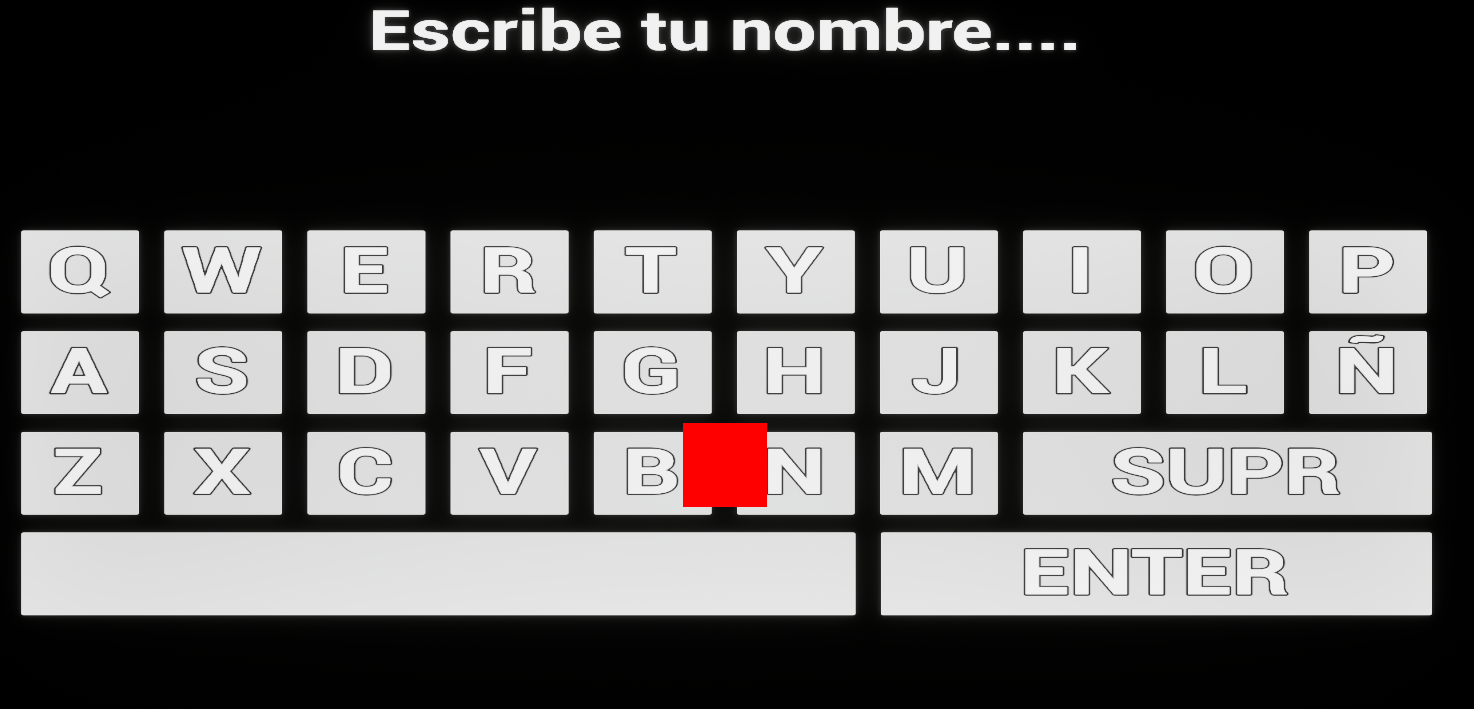
\includegraphics[width=\textwidth]{../img/anexos/Pantalla_De_Registro.png}
    \caption[Pantalla de registro]{Pantalla de registro.}
	\label{b:pantalla_registro}
\end{figure}

\subsection{Crear nueva partida}
Para crear una nueva partida, hay que seguir estos pasos:
\begin{enumerate}
    \item Acceder a la pantalla de menú principal ~\ref{b:pantalla_menu_principal}.
    \item Presionar el botón de  Nueva partida para entrar en la pantalla de nuevo puzle ~\ref{b:pantalla_nuevo_puzle}.
    \item Presionar el puzle que desees jugar.
    
\end{enumerate}
\begin{figure}[h]
	\centering
	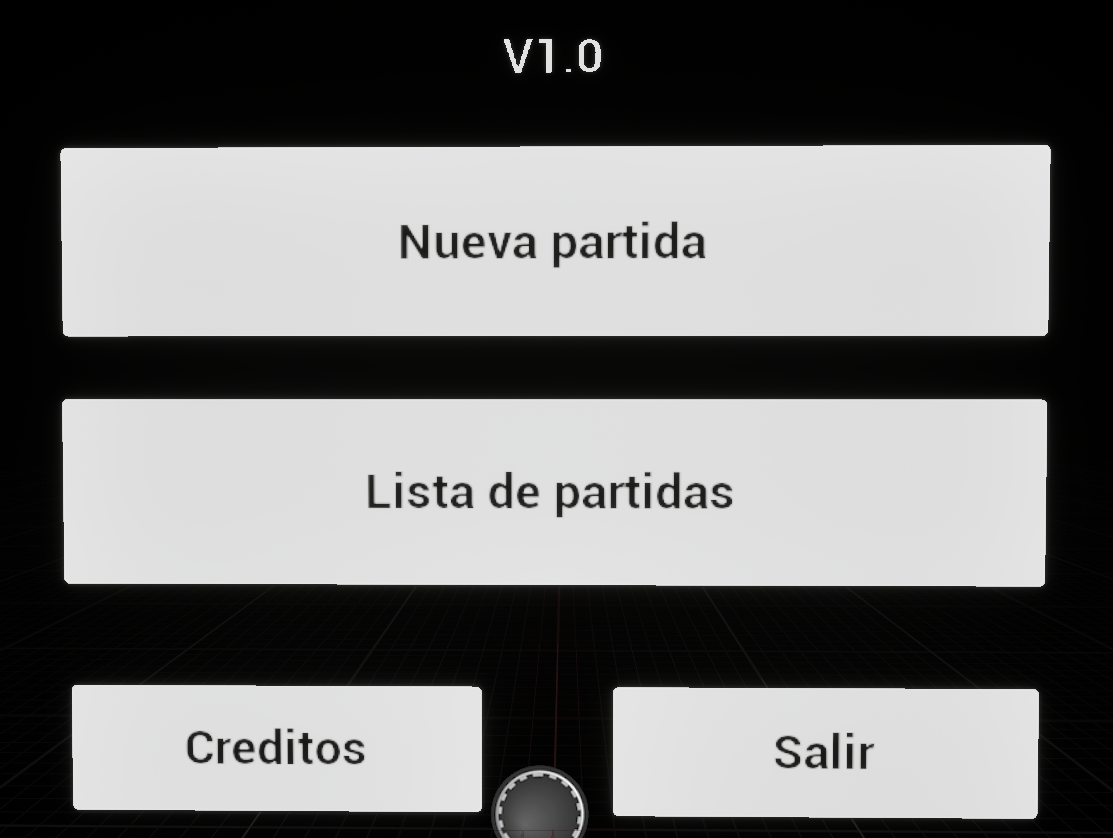
\includegraphics[width=\textwidth]{../img/anexos/pantalla_menu_principal.png}
    \caption[Pantalla de registro]{Pantalla de menú principal.}
	\label{b:pantalla_menu_principal}
\end{figure}

\begin{figure}[h]
	\centering
	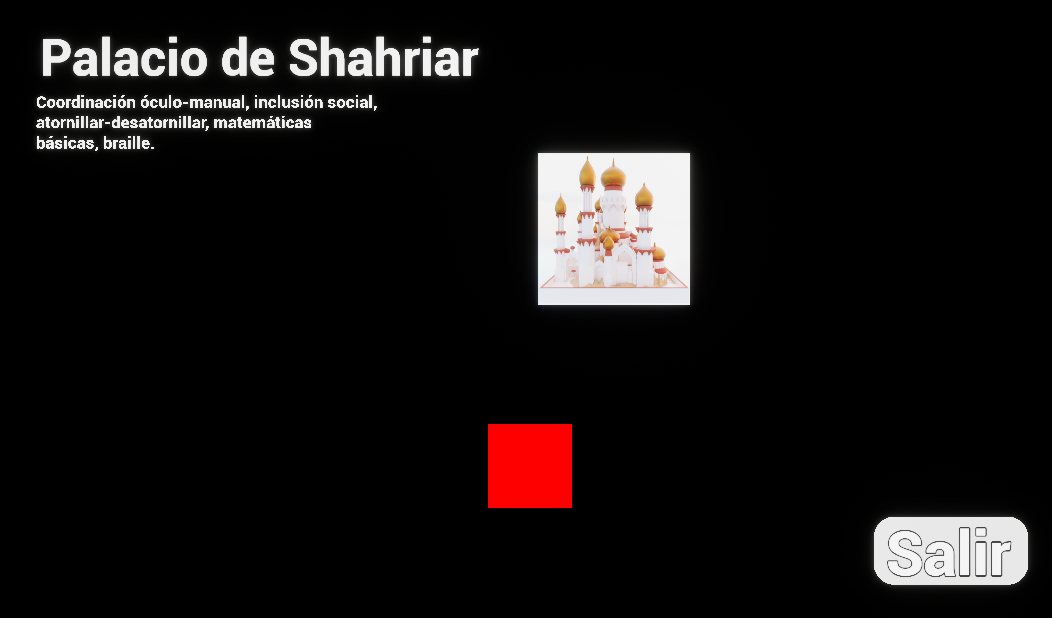
\includegraphics[width=\textwidth]{../img/anexos/pantalla_nuevo_puzle.png}
    \caption[Pantalla de registro]{Pantalla de nuevo puzle.}
	\label{b:pantalla_nuevo_puzle}
\end{figure}

\subsection{Borrar partida}
Para borrar una partida, hay que seguir estos pasos:
\begin{enumerate}
    \item Acceder a la pantalla de menú principal ~\ref{b:pantalla_menu_principal}
    \item Presionar el botón de  ``Lista de partidas'' para entrar en la pantalla de listado de partidas ~\ref{b:pantalla_listado_puzles}.
    \item Presionar el botón de borrar del puzle que desees borrar.
\end{enumerate}

\begin{figure}[h]
	\centering
	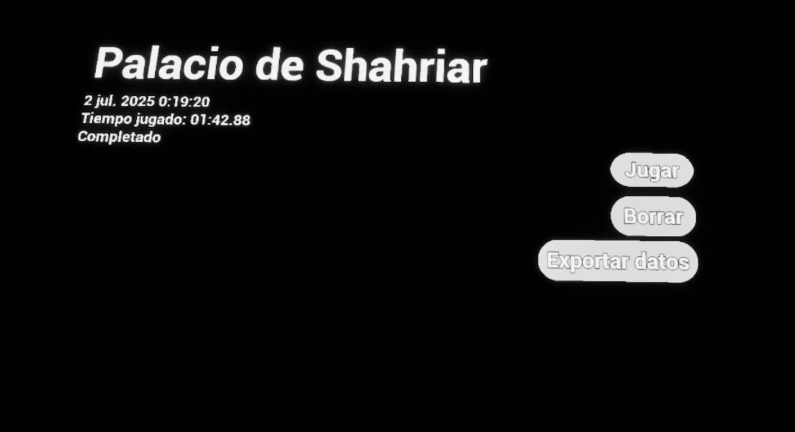
\includegraphics[width=\textwidth]{../img/anexos/pantalla_listado_puzles.png}
    \caption[Pantalla de listado de puzles]{Pantalla de listado de puzles.}
	\label{b:pantalla_listado_puzles}
\end{figure}

\subsection{Cargar partida}
Para cargar una partida, hay que seguir estos pasos:
\begin{enumerate}
    \item Acceder a la pantalla de menú principal ~\ref{b:pantalla_menu_principal}
    \item Presionar el botón de  ``Lista de partidas''  para entrar en la pantalla de listado de partidas ~\ref{b:pantalla_listado_puzles}.
    \item Presionar el botón de jugar del puzle que desees jugar.
\end{enumerate}

\subsection{Exportar datos de partida}
Para cargar una partida, hay que seguir estos pasos:
\begin{enumerate}
    \item Acceder a la pantalla de menú principal ~\ref{b:pantalla_menu_principal}
    \item Presionar el botón de  ``Lista de partidas``para entrar en la pantalla de listado de partidas ~\ref{b:pantalla_listado_puzles}.
    \item Presionar el botón de exportar datos del puzle que desees exportar.
    \item Ir a la carpeta donde tengas descargado el programa e ir a ``Windows $\rightarrow$ TFG''.
    \item Abrir con una hoja de calculo el archivo datos \texttt{``datos\_puzle\_exportado.csv''}.
\end{enumerate}

